\documentclass[10pt]{article}

\usepackage[margin=1in]{geometry}
\usepackage{amsmath}
\usepackage{amssymb}
\usepackage{amsthm}
\usepackage{mathtools}
\usepackage{bm}

\usepackage{color}
\usepackage{colortbl}
\definecolor{deepblue}{rgb}{0,0,0.5}
\definecolor{deepred}{rgb}{0.6,0,0}
\definecolor{deepgreen}{rgb}{0,0.5,0}
\definecolor{gray}{rgb}{0.7,0.7,0.7}

\usepackage{hyperref}
\hypersetup{
  colorlinks   = true, %Colours links instead of ugly boxes
  urlcolor     = black, %Colour for external hyperlinks
  linkcolor    = blue, %Colour of internal links
  citecolor    = blue  %Colour of citations
}

%%%%%%%%%%%%%%%%%%%%%%%%%%%%%%%%%%%%%%%%%%%%%%%%%%%%%%%%%%%%%%%%%%%%%%%%%%%%%%%%

\theoremstyle{definition}
\newtheorem{problem}{Problem}
\newtheorem{defn}{Definition}
\newcommand{\R}{\mathbb R}
\DeclareMathOperator{\vcdim}{VCdim}
\DeclareMathOperator{\E}{\mathbb E}
\DeclareMathOperator{\nnz}{nnz}
\DeclareMathOperator{\determinant}{det}
\DeclareMathOperator{\Var}{Var}
\DeclareMathOperator{\rank}{rank}
\DeclareMathOperator*{\argmin}{arg\,min}
\DeclareMathOperator*{\argmax}{arg\,max}

\newcommand{\I}{\mathbf I}
\newcommand{\Q}{\mathbf Q}
\newcommand{\p}{\mathbf P}
\newcommand{\pb}{\bar {\p}}
\newcommand{\pbb}{\bar {\pb}}
\newcommand{\pr}{\bm \pi}
\newcommand{\epsapp}{\epsilon_{\text{app}}}
\newcommand{\epsest}{\epsilon_{\text{est}}}

\newcommand{\trans}[1]{{#1}^{T}}
\newcommand{\loss}{\ell}
\newcommand{\w}{\mathbf w}
\newcommand{\x}{\mathbf x}
\newcommand{\y}{\mathbf y}
\newcommand{\lone}[1]{{\lVert {#1} \rVert}_1}
\newcommand{\ltwo}[1]{{\lVert {#1} \rVert}_2}
\newcommand{\lp}[1]{{\lVert {#1} \rVert}_p}
\newcommand{\linf}[1]{{\lVert {#1} \rVert}_\infty}
\newcommand{\lF}[1]{{\lVert {#1} \rVert}_F}

\newcommand{\h}{\mathcal H}
\newcommand{\D}{\mathcal D}
\DeclareMathOperator*{\erm}{ERM}

%%%%%%%%%%%%%%%%%%%%%%%%%%%%%%%%%%%%%%%%%%%%%%%%%%%%%%%%%%%%%%%%%%%%%%%%%%%%%%%%

\begin{document}


\begin{center}
\Huge
Notes: Statistical Learning Theory II
\end{center}

\begin{center}
%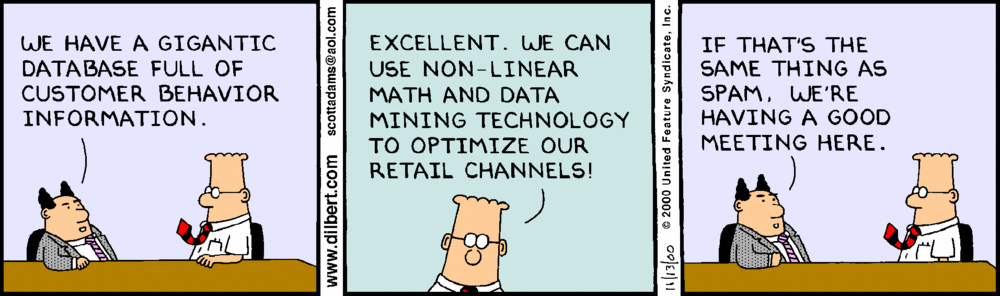
\includegraphics[width=\textwidth]{dilbert}
%
    %\vspace{0.2in}
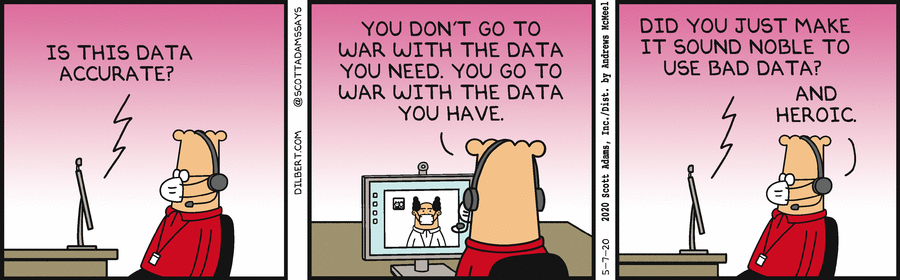
\includegraphics[width=\textwidth]{dt200507}

\end{center}

\section{Pre-lecture Work}

\begin{problem}
    (optional)
    Chapter 4 of Shalev-Shwartz and Ben-David covers a concept called \emph{uniform convergence}.
    This is a mathematical tool that was historically used before the discovery of the VC-dimension,
    and is currently used in situations where the VC-dimension is not applicable.
    We will not cover the concept in this class,
    but if you are particularly interested in machine learning theory,
    then I recommend reading section 4.1 from this chapter.
    (It's only 2 pages.)
    Then in Section 4.2, the authors generalize Corollary 2.3 (finite hypothesis classes are PAC learnable) to the agnostic setting.
    %Our discussion of VC-dimension below further generalizes this result,
    %so there is no need to know the results in this section.
\end{problem}

\begin{problem}
    Read Chapter 5 of Shalev-Shwartz and Ben-David.
    (You may skip section 5.1, which formally defines the \emph{No Free Lunch Theorem}.)
    Complete the following notes as you read.
    \begin{enumerate}
        %\item No Free Lunch Theorem (Theorem 5.1)
        %\item Corollary 5.2
        \item Equation (5.7)
            \vspace{3in}
        %\item Approximation Error
            %\vspace{3in}
        %\item Estimation Error
            %\vspace{3in}
    \end{enumerate}
\end{problem}

\newpage
\begin{problem}
    Read Chapter 6 of Shalev-Shwartz and Ben-David.
    (You may skip Section 6.5, which is only concerned with proofs.)
    Complete the following notes as you read.
    \begin{enumerate}
        \item Restriction of $\mathcal H$ to $C$ (Definition 6.2)
            \vspace{4in}
        \item Shattering (Definition 6.3)
            \vspace{4in}
        \item VC-Dimension (Definition 6.5)
            \vspace{4.5in}
        \item Theorem 6.6
            \vspace{4.5in}
        \item The Fundamental Theorem of Statistical Learning (Theorem 6.7).
            You may ignore result 1 about uniform convergence
            (we're not covering uniform convergence in this class).
            You only need to know results 2-6.
            \vspace{4in}
        \item The Fundamental Theorem of Statistical Learning - Quantitative Version (Theorem 6.8).
            You may ignore result 1 about uniform convergence
            (we're not covering uniform convergence in this class).
            You only need to know results 2 and 3 about PAC and agnostic PAC learnability.
            \vspace{4in}
    \end{enumerate}
\end{problem}

\newpage
\begin{problem}
    For each hypothesis class below,
    formally define the hypothesis class and state its VC-dimension.
    You can find all of these answers in Section 6.3.
    You do not need to provide the proof of the VC-dimension below.
    %but you should be able to understand the proof presented in the book.
    \begin{enumerate}
        \item Threshold functions
            \vspace{4.5in}
        \item Intervals
            \vspace{4.5in}
        \item Axis Aligned Rectangles
            \vspace{4.5in}
        \item Finite Classes
            \vspace{4.5in}
    \end{enumerate}
\end{problem}

\begin{problem}
    Prove or disprove the following statements.
    Note that all of the proofs/disproofs follow immediately from the definitions above, and that is why they are included in this section.
    You do not have to complete all of these problems before the start of lecture.
    We will discuss some of these problems during lecture,
    but I recommend you solve as many as you can on your own before lecture.

    \begin{enumerate}
        \item
            The following equation always holds:
            \begin{equation}
                L_\mathcal D(h_S) - \epsest = \epsapp
            \end{equation}
            \vspace{2.25in}
        \item
            The following equation always holds:
            \begin{equation}
                L_\mathcal D(h_S) - \min_{h\in\mathcal H} L_\mathcal D(h) = \epsest
            \end{equation}
            \vspace{2.25in}
        \item
            The following equation always holds:
            \begin{equation}
                \epsapp>0
            \end{equation}
            \vspace{2.75in}
        \item
            The following equation always holds:
            \begin{equation}
                \epsest>0
            \end{equation}
            \vspace{2.75in}
        \item
            The following equation always holds:
            \begin{equation}
                \epsest<\epsapp
            \end{equation}
            \vspace{2.75in}
        \item
            As the number of data points in the training set increases,
            the approximation error decreases.
            \vspace{2.75in}
        \item
            Let $\mathcal H_1$ and $\mathcal H_2$ be hypothesis classes where $\mathcal H_1 \subset \mathcal H_2$.
            Then, the approximation error of $\mathcal H_1$ is greater than or equal to the approximation error of $\mathcal H_2$.
            \vspace{2.75in}

        \item
            Let $\mathcal H_1$ and $\mathcal H_2$ be hypothesis classes where $\mathcal H_1 \subset \mathcal H_2$.
            Then, the estimation error of $\mathcal H_1$ is less than or equal to the estimation error of $\mathcal H_2$.
            \vspace{2.75in}

        \item
            A model with a high approximation error and a low estimation error is underfitting.
            \vspace{2.75in}

        \item
            A model with a low approximation error and a high estimation error is overfitting.
            \vspace{2.75in}

        \item 
            If $\vcdim(\mathcal H)$ is finite,
            then $\epsapp=0$.
            \vspace{2.75in}
        \item 
            If $\vcdim(\mathcal H)$ is infinite,
            then $\epsapp=0$.
            \vspace{2.75in}
        \item
            If $\vcdim(\mathcal H)$ is finite,
            then the Bayes optimal predictor $f_\mathcal D \in \mathcal H$.
            \vspace{2.75in}

        \item
            If $\vcdim(\mathcal H)$ is infinite,
            then the Bayes optimal predictor $f_\mathcal D \not \in \mathcal H$.
            \vspace{2.75in}

        \item
            If $\vcdim(\mathcal H)$ is infinite,
            then $L_\mathcal D(h) > 0$ for all distributions $\mathcal D$, datasets $S\sim\mathcal D^m$, and $h\in\mathcal H$.
            \vspace{2.75in}

        \item
            If $\vcdim(\mathcal H)$ is infinite,
            then $L_S(h_S) = 0$ for all distributions $\mathcal D$, datasets $S\sim\mathcal D^m$, and any ERM $h_S\in\mathcal H$.
            \vspace{2.75in}

        \item
            If $\vcdim(\mathcal H)$ is finite,
            then $\mathcal H$ is PAC learnable.
            \vspace{2.75in}

        \item
            If $\mathcal H$ is agnostic PAC learnable, then it is also PAC learnable.
            \vspace{2.75in}

        %\item
            %Let $\vcdim(\mathcal H) = \infty$ and .
            %then there exists a distribution $\mathcal D$ such that
            %\begin{equation}
            %\end{equation}

        \item
            For every two hypotheses class $\mathcal H_1$ and $\mathcal H_2$,
            if $\mathcal H_1 \subset \mathcal H_2$, than $\vcdim(\mathcal H_1) \le \vcdim(\mathcal H_2)$.
            \vspace{2.75in}

        \item
            For every two hypotheses class $\mathcal H_1$ and $\mathcal H_2$,
            if $\vcdim(\mathcal H_1) = \vcdim(\mathcal H_2)$,
            then $\mathcal H_1 = \mathcal H_2$.
            \vspace{2.75in}

        \item
            The ordinary least squares (OLS) hypothesis class discussed in the previous lecture notes has a finite VC dimension.
            \vspace{2.75in}
    \end{enumerate}
\end{problem}

%%%%%%%%%%%%%%%%%%%%%%%%%%%%%%%%%%%%%%%%%%%%%%%%%%%%%%%%%%%%%%%%%%%%%%%%%%%%%%%%

\newpage
\section{Lecture}


\begin{problem}
    Combine Theorem 6.8 and the definition of (agnostic) PAC learnability to bound the generalization error of a hypothesis class based on its VC-dimension.
\end{problem}

\newpage
\begin{problem}
    Linear models are one of the main tools in data mining.
    Chapter 9 in Shalev-Swartz and Ben-David discuss linear predictors in significantly more detail than we need for this class.
    In this problem, we will review all the relevant concepts.
    \begin{enumerate}
        \item Define the hypothesis class of halfspaces.
            \vspace{5in}
        \item What is separability?
            \vspace{0.8in}
        \item What is the VC-Dimension?
            \vspace{0.8in}
        \item What is the computational complexity of computing the ERM in the separable and agnostic cases?
            \vspace{0.8in}
    \end{enumerate}
\end{problem}

%\begin{problem}
    %Logistic regression.
    %\begin{enumerate}
        %\item State and draw the logistic function.
        %\item 
    %\end{enumerate}
%\end{problem}

\begin{problem}
    Kernel functions are tools that let us manipulate the VC-dimension of hypothesis classes.
    They also have nice computational properties,
    but in this problem we are only concerned with their statistical properties.
    \begin{enumerate}
        \item Define the polynomial kernel. 
            \vspace{4.5in}
        \item What is the VC-dimension of halspaces with the polynomial kernel?
            \vspace{2in}
        \item When would we use the polynomial kernel?
            \newpage
        \item Define the random projection kernel.
            \vspace{4.5in}
        \item What is the VC-dimension of halspaces with the random projection kernel?
            \vspace{2in}
        \item When would we use the random projection kernel?
    \end{enumerate}
\end{problem}

%\begin{problem}
    %Projected linear classifier.
%\end{problem}
%
%\begin{problem}
    %Neural networks.
%\end{problem}
%
%\begin{problem}
    %Nearest neighbor.
%\end{problem}
%
%\begin{problem}
    %Ensemble methods.
%\end{problem}

\end{document}


